\hypertarget{vo_8cpp}{}\section{/home/bhargavi/\+Documents/\+S\+D\+R/\+Copy\+\_\+\+Exam\+\_\+808\+X/app/vo.cpp File Reference}
\label{vo_8cpp}\index{/home/bhargavi/\+Documents/\+S\+D\+R/\+Copy\+\_\+\+Exam\+\_\+808\+X/app/vo.\+cpp@{/home/bhargavi/\+Documents/\+S\+D\+R/\+Copy\+\_\+\+Exam\+\_\+808\+X/app/vo.\+cpp}}


E\+N\+P\+M808X, Mid\+Sem Exam.  


{\ttfamily \#include $<$vo.\+hpp$>$}\\*
Include dependency graph for vo.\+cpp\+:\nopagebreak
\begin{figure}[H]
\begin{center}
\leavevmode
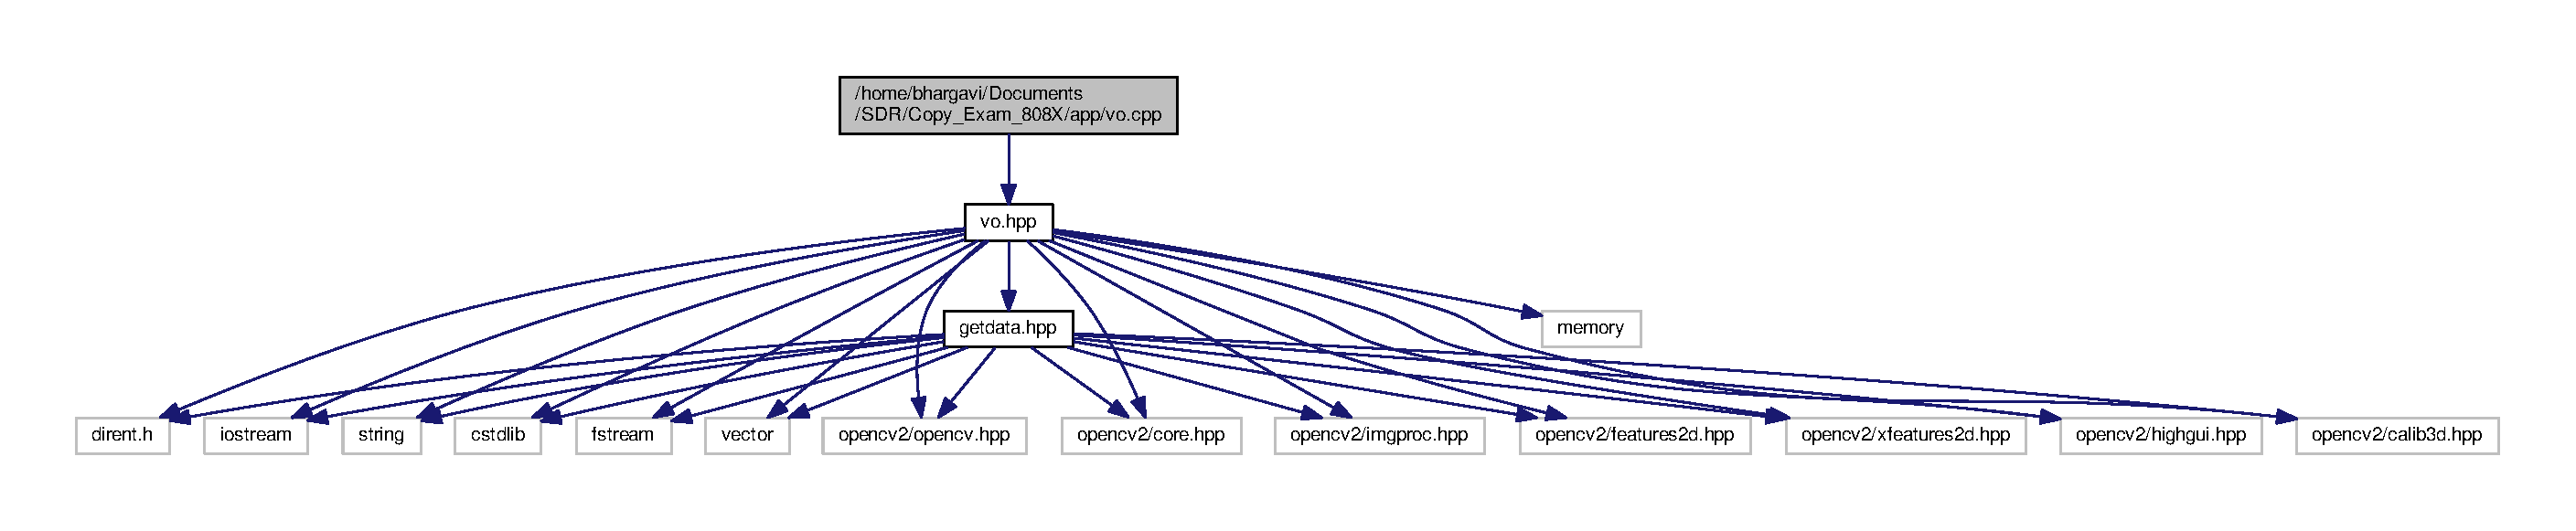
\includegraphics[width=350pt]{vo_8cpp__incl}
\end{center}
\end{figure}


\subsection{Detailed Description}
E\+N\+P\+M808X, Mid\+Sem Exam. 

\begin{DoxyAuthor}{Author}
Bhargavi Patel 
\end{DoxyAuthor}
\begin{DoxyCopyright}{Copyright}
M\+IT License
\end{DoxyCopyright}
\hypertarget{votest_8cpp_DESCRIPTION}{}\subsection{D\+E\+S\+C\+R\+I\+P\+T\+I\+ON}\label{votest_8cpp_DESCRIPTION}
This is the main implementation of visual odometry code.\+It is taking sequence of images as input and calculating the rotational and trasnalational parameters according to camera centre considering and comparing features.\+I am using S\+U\+RF features as they are faster than S\+H\+IF features.\+The image is preproced in many ways and denoising is also done before comparing the features. 